% !TEX TS-program = pdflatex
% !TEX encoding = UTF-8 Unicode

% This is a simple template for a LaTeX document using the "article" class.
% See "book", "report", "letter" for other types of document.

\documentclass[12pt]{article} % use larger type; default would be 10pt
\usepackage[utf8]{inputenc}   % set input encoding (not needed with XeLaTeX)

%%% PAGE DIMENSIONS
\usepackage{geometry}
\geometry{letterpaper}
\geometry{margin=1in} % 1in page margin

%%% COLOR AND GRAPHICS
\usepackage{color}
\usepackage{graphicx} % support the \includegraphics command and options

\usepackage{pslatex}
\definecolor{mygreen}{rgb}{0,0.6,0}
\definecolor{mygray}{rgb}{0.5,0.5,0.5}
\definecolor{mymauve}{rgb}{0.58,0,0.82}
\usepackage{listings} % For displaying source code
\lstset{ %
	language=C,                      % the language of the code
	backgroundcolor=\color{white},   % choose the background color; you must add \usepackage{color} or \usepackage{xcolor}
	basicstyle=\sffamily\fontsize{11}{13.2}\selectfont,        % the size of the fonts that are used for the code
	breakatwhitespace=false,         % sets if automatic breaks should only happen at whitespace
	breaklines=true,                 % sets automatic line breaking
	captionpos=t,                    % sets the caption-position to bottom
	commentstyle=\color{mygreen},    % comment style
	deletekeywords={...},            % if you want to delete keywords from the given language
	escapeinside={\%*}{*)},          % if you want to add LaTeX within your code
	extendedchars=true,              % lets you use non-ASCII characters; for 8-bits encodings only, does not work with UTF-8
	frame=single,                    % adds a frame around the code
	keepspaces=true,                 % keeps spaces in text, useful for keeping indentation of code (possibly needs columns=flexible)
	keywordstyle=\color{blue},       % keyword style
	morekeywords={*,...},            % if you want to add more keywords to the set
	numbers=left,                    % where to put the line-numbers; possible values are (none, left, right)
	numbersep=5pt,                   % how far the line-numbers are from the code
	numberstyle=\color{mygray},      % the style that is used for the line-numbers
	rulecolor=\color{black},         % if not set, the frame-color may be changed on line-breaks within not-black text (e.g. comments (green here))
	showspaces=false,                % show spaces everywhere adding particular underscores; it overrides 'showstringspaces'
	showstringspaces=false,          % underline spaces within strings only
	showtabs=false,                  % show tabs within strings adding particular underscores
	stepnumber=1,                    % the step between two line-numbers. If it's 1, each line will be numbered
	stringstyle=\color{mymauve},     % string literal style
	tabsize=2,                       % sets default tabsize to 2 spaces
	title=\lstname                   % show the filename of files included with \lstinputlisting; also try caption instead of title
}

% \usepackage[parfill]{parskip} % Activate to begin paragraphs with an empty line rather than an indent

%%% PACKAGES
\usepackage{booktabs} % for much better looking tables
\usepackage{array}    % for better arrays (eg matrices) in maths
\usepackage{paralist} % very flexible & customisable lists (eg. enumerate/itemize, etc.)
\usepackage{verbatim} % adds environment for commenting out blocks of text & for better verbatim
%\usepackage{subfig}   % make it possible to include more than one captioned figure/table in a single float
\usepackage{subcaption}
\usepackage{adjustbox}
\usepackage{placeins} % allows for use of \FloatBarrier to prevent floats from moving past line.

%%% HEADERS & FOOTERS
%\usepackage{fancyhdr} % This should be set AFTER setting up the page geometry
%\pagestyle{fancy} % options: empty , plain , fancy
%\renewcommand{\headrulewidth}{0pt} % customise the layout...
%\lhead{}\chead{}\rhead{}
%\lfoot{}\cfoot{\thepage}\rfoot{}


%%% SECTION TITLE APPEARANCE
\usepackage{sectsty}
\sectionfont{\normalsize\bfseries\uppercase}
\subsectionfont{\normalsize\bfseries}
\subsubsectionfont{\normalsize\mdseries\itshape}

%%% ToC (table of contents) APPEARANCE
\usepackage[nottoc,notlof,notlot]{tocbibind} % Put the bibliography in the ToC
\usepackage[titles]{tocloft} % Alter the style of the Table of Contents
\renewcommand{\cftsecfont}{\rmfamily\mdseries\upshape}
\renewcommand{\cftsecpagefont}{\rmfamily\mdseries\upshape} % No bold!

%%% Title setup
\newcommand{\TitleFont}{\fontsize{16}{20}\selectfont\bfseries}
\newcommand{\AuthorFont}{\fontsize{14}{17}\selectfont}

%%% END Article customizations

%%% The "real" document content comes below...

\title{\TitleFont EE 478 Capstone Final Report \\ RFID Interaction Suite \vfill }
\author{\AuthorFont Alyanna Castillo \\ Patrick Ma \\ Ryan McDaniels}
\date{}

\begin{document}

%% Make title and ToC, start page numbering AFTER ToC
\maketitle
\thispagestyle{empty}
\pagebreak \tableofcontents
\listoftables
\listoffigures
\thispagestyle{empty}
\pagebreak
\setcounter{page}{1}

\section{Abstract}
% The abstract should provide a brief overview of the report.  It should provide
% a summary of the main specific points for the introduction, the main tests and
% experiments, the results, and the conclusions. It is called an abstract because
% you can literally "abstract" sentences from the other sections. 
% 
% Once again, this is not a narrative of your experiences as you executed the
% design.  The abstract should mirror (albeit in a very condensed way) the
% content of your report.

\section{Introduction}
% Brief introduction and overview of the purpose of the lab and of the methods
% and tools used.


% This section should include the following:

\textbf{These are some example of how to cite and use bullet points}
A reference to Table~\ref{tab:bomTable} and one to the Design Specification, Section~\ref{sec:designSpec}.

\begin{itemize}
	\item Overall summary description of the module - 2-3 paragraphs maximum
		(explanation of use cases goes here)

		\begin{itemize}
			\item Specification of the public interface to the module

				\begin{itemize}
					\item Inputs
					\item Outputs
					\item Side effects
				\end{itemize}

			\item Psuedo English description of algorithms, functions, or procedures
			\item Timing constraints
			\item Error handling
		\end{itemize}
\end{itemize}


\section{Design Specification}\label{sec:designSpec} 
% In this subsection you will textually describe your client's requirements.
% What does he or she need in the project you are developing.  If you are
% incorporating extra features or capabilities, please describe them clearly in
% this section.

\subsubsection{Design Overview}
This system is a RFID-based gaming system. A user is able to play alone against a computer, or can play with other users owning a system using a multiplayer connection feature. Additionally, users can create their own customized cards using a third built-in function of the device.

\subsection{Design Requirements}\label{sec:requirements} % Patrick , additions by Alyanna, Ryan
\subsubsection{Environmental Requirements}

The device must operate in an indoor/outdoor environment with relative
humidity consistent with desert and tropical environments. It must be durable
enough to withstand various types of users, especially small children.  The
unit is to be portable and battery operated.

\subsubsection{System Input and Output Requirements}

The system must be capable of accepting several different types of signals and inputs:

\begin{itemize}
	\item Standard frequencies used for close-range or Near-Field Communication Radio Frequency Identification (RFID) devices
	\item Standard frequencies used for commercial wireless communication standards such as wifi networks
	\item User input from a keypad to navigate menus, enter commands, and provide other alphanumeric information
	\item When in multiplayer mode, communication and commands from other players must be accepted and responded to.
\end{itemize}

The system must be capable of providing the following outputs:
\begin{itemize}
	\item Display information about the current game state through an LCD screen
	\item Provide status information of individual cards placed on the game board
	\item Send commands to other systems when in multiplayer mode
	\item Send wireless signals to program RFID-enabled cards
\end{itemize}

\subsubsection{User Interface}

The system must support the following modes of operation:

\begin{description}
	\item[Single Player:] Allows the user to select from, and play, single player games. Upon entering Single Player mode, the system prompts the user to select a game to play from those stored in memory. Selecting a valid game loads the game from memory and begins game execution.
	\item[Multiplayer:] Allows the user to select and play multiplayer games. Upon entering Multiplayer mode, the system activates wireless communication and attempts to connect to other users in Multiplayer mode. Once a connection is established, the users select a multiplayer game on both systems and gameplay begins.
	\item[Build Card:] Allows the user to create custom cards for a game. The data stored will vary based on game requirements. All cards must contain unique card serial numbers or identifing ID numbers, and a code that specifies which games the card is valid for.
\end{description}

The system must also have the following buttons, switches or interface devices:

\begin{itemize}
	\item 16-button keypad with alphanumeric character labels
	\item Reset button that when pressed causes a soft reset of the system
	\item Power button that turns the system on and off
	\item An LCD screen viewable from several angles. The screen must be viewable indoors and in overcast conditions
\end{itemize}

\subsection{Identified Use Cases}\label{sec:identifiedUseCases} % Alyanna

\subsection{Detailed Specifications}\label{detailedSpec} % Ryan

\subsection{Functional Decomposition}\label{functions} % Patrick

\section{Hardware Implementation}\label{hwImplementation} 

\subsection{Top Level Design}\label{hwTopLevel} % Patrick

\subsection{Low Level Design}\label{hwLowLevel} % Patrick

\section{Software Implementation}\label{swImplementation}
%
%What is your design????
%
%Present your design starting from a top level functional view and potentially
%block diagram or high level architecture.  Refine that view to present and
%explain each of the modules that comprise the major functional blocks.  Discuss
%the flow of control through the design.  Identify and discuss the specific
%processes/tasks you have implemented in your design. Explain your design
%choices.    

\subsection{Top Level Design}\label{swTopLevel} % Alyanna
%
%Put stuff here about the functional decomposition, system architecture,
%interaction of parts.

\subsection{Low Level Design}\label{swLowLevel} % Alyanna
%
%task level implementation details here. Control diagram goes here, etc.

\section{Presentation, Discussion, and Analysis of the Results}
%
%Based upon the execution of your design, present your results. Explain them and
%what was expected, and draw any conclusions (for example, did this prove your
%design worked).
%
%In addition to a detailed discussion and analysis of your project and your
%results, you must include all the answers to all questions raised in the lab.
\subsection{Results } % Ryan

\subsection{Discussion of Results } % Alyanna

\subsection{Analysis of Any Errors } % Ryan
%
%This one is obvious. Do this section as appropriate.  If it improves the flow,
%it does not need to be a separate section and may be included in the
%presentation, discussion, and analysis of the results.  However, it will still
%be graded separately and must be present.

\subsection{Analysis of Implementation Issues and Workarounds} % Patrick
%
%State any problems you encountered while working on the project. If your
%project did not work or worked only partially, provide an analysis of why and
%what efforts were made to identify the root cause of any problems. \\
%

\section{Test Plan } % Ryan
%
%Overall summary of what needs to be tested to ensure that your design meets the
%original requirements, 2-3 paragraphs maximum unless specified otherwise

\subsection{Test Specification} % Patrick
%
%Annotated description of what is to be tested and the test limits.  This
%specification quantifies inputs, outputs, and constraints on the system.  That
%is, it provides specific values for each. 
%
%Note, this does not specify test implementation...this is what to do, not how
%to do it.

\subsection{Test Cases} % Alyanna
%
%Annotated description of how your system is to be tested against the test
%limits
%Note, this does specify test implementation...this is not what to do, this is
%how to do it based upon the test specification.

\section{Summary and Conclusion}
%
%You should know these sections very well, no need to explain.  Note, however,
%that they are two different sections.  The summary is just that, a summary of
%your project.  It should loosely mirror the abstract with a bit more detail.
%The conclusion concludes the report, potentially adds information that is often
%outside the main thrust of the report, and may offer suggestions or
%recommendations about the project.

\subsection{Final Summary}


\subsection{Project Conclusions} % Patrick, Alyanna, Ryan
% Include comments and reflections on the capstone. What went well, what could
% be improved next time, What was enjoyable and/or challenging.


\pagebreak
\appendix


\section{Breakdown of Lab Person-hours (Estimated)}
% Use the '&' to separate columns
\begin{tabular}{|l|*{4}{r|}}
	\hline
	Person & Design Hrs & Code Hrs & Test/Debug Hrs & Documentation Hrs \\ \hline
	Patrick & x & x & x & x  \\ \hline
	Alyanna & x & x & x & x \\ \hline
	Ryan & x & x & x & x  \\ \hline
\end{tabular}

~\\

By initializing/signing above, I attest that I did in fact work the
estimated number of hours stated. I also attest, under penalty of shame,
that the work produced during the lab and contained herein is actually my
own (as far as I know to be true). If special considerations or
dispensations are due others or myself, I have indicated them below.

\pagebreak

%\section{Bill of Materials\label{appendix:bom}}
%Table~\ref{tab:bomTable} lists the bill of materials for the construction of one system.
%
%\begin{table}[h]
%	\begin{tabular}{llll}
%		\multicolumn{4} {c} {\textbf{Bill of Materials}} \\
%		\toprule
%		\textbf{Item}                         & \textbf{Unit Cost} & \textbf{Quantity} & \textbf{Total Cost} \\ \midrule
%		TI HI-Plus RFID Tags                  & 0.91          & 20                & 18.20               \\
%		DLP-RFID2 RFID Reader/Writer          & 50            & 3                 & 150                 \\
%		Xbee S1 Wireless Chips                & 30            & 2                 & 60                  \\
%		PLA Makerbot Filament                 & 48            & 1                 & 48                  \\
%		GAL22V10D                             & 3.5           & 4                 & 14                  \\
%		PICKit 3                              & 45            & 2                 & 90                  \\
%		CY7C128A SRAM                         & 4             & 2                 & 8                   \\
%		3.3 Volt Linear Regulator             & 3.22          & 2                 & 6.44                \\
%		Lever Switch, micro SPDT, momentary   & 2.5           & 6                 & 15                  \\
%		16-key Numeric Keypad                 & 7.5           & 2                 & 15                  \\
%		128x169 Color LCD                     & 17            & 2                 & 34                  \\
%		PIC18F46K22 Microcontrollers          & 7.7           & 4                 & 30.8                \\
%		RGB LED, Common Cathode               & 4             & 8                 & 12                  \\
%		(EXTRA)                               &               &                   &                     \\
%		(EXTRA)                               &               &                   &                     \\
%		(EXTRA)                               &               &                   &                     \\ \bottomrule
%		Total Cost                            &               &                   &                    
%	\end{tabular}
%	\caption{\label{tab:bomTable}}
%\end{table}
%
%\FloatBarrier
%\section{Hardware Diagrams\label{appendix:hwDiagrams}}
%\begin{figure}[H]
%	\centering
%	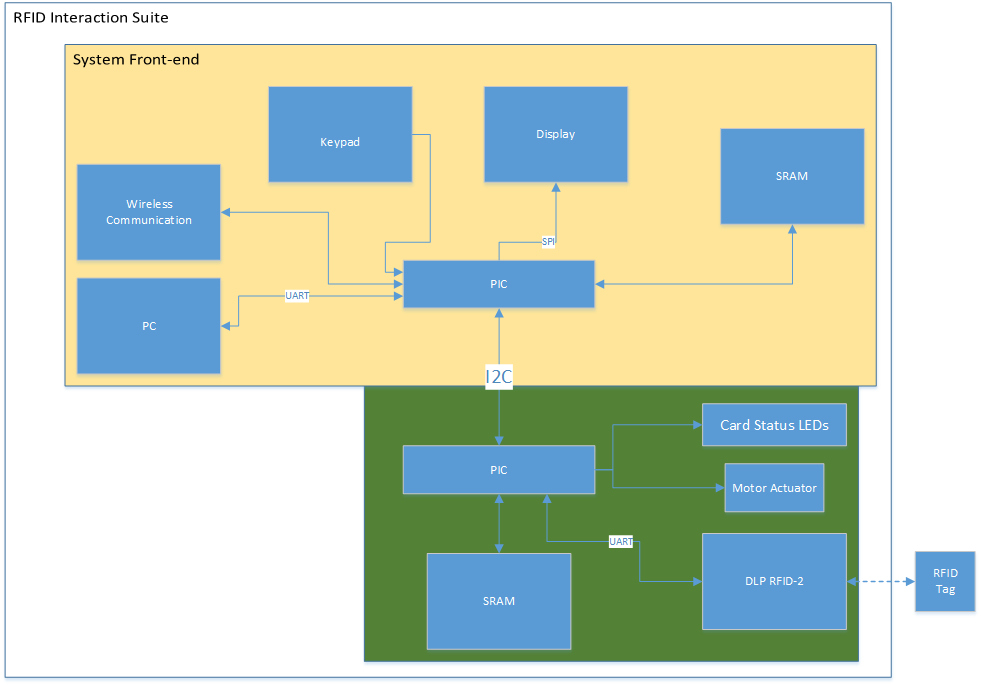
\includegraphics[width=\textwidth]{images/BlockDiagram.png}
%	\caption{High level block diagram of the system hardware components}
%	\label{fig:highLevelBlockDiagram}
%\end{figure}
%
%\begin{figure}[H]
%	\centering
%	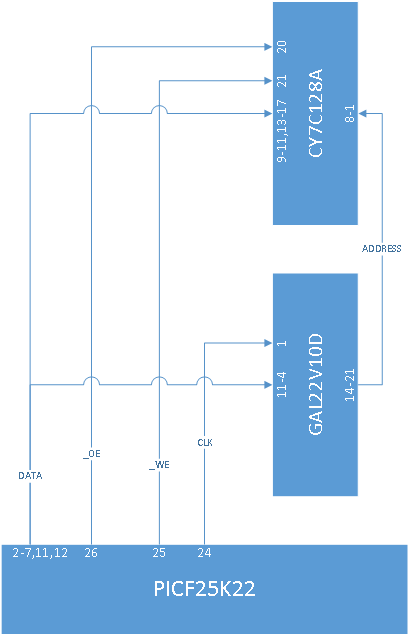
\includegraphics[width=0.8\textwidth]{images/SRAMHardwareBlock.png}
%	\caption{Block diagram of the SRAM hardware system}
%	\label{fig:sramBlockDiagram}
%\end{figure}
%
%\begin{figure}[H]
%	\centering
%	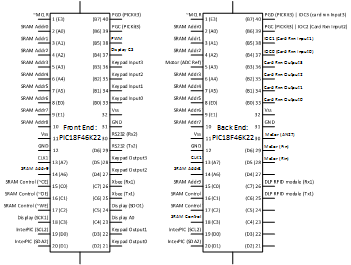
\includegraphics[height=4in]{images/PinOuts.png}
%	\caption{Pinouts to the front- and back-end microcontrollers}
%	\label{fig:pinoutDiagram}
%\end{figure}
%
%\FloatBarrier
%\section{Functional Decomposition Diagram\label{fig:funcDecomp}}
%
%\begin{figure}[H]
%	\centering
%	\includegraphics[width=\textwidth]{images/funDecomp.png}
%	\caption{Software functional decomposition showing the major functional divisions and tasks}
%	\label{fig:funDecomp}
%\end{figure}
%
%\FloatBarrier
%\section{State Diagrams}
%\FloatBarrier
%\subsection{System State Diagram\label{fig:sysStateDiagram}}
%\begin{figure}[H]
%	\centering
%	\begin{subfigure}{0.48\textwidth}
%		\includegraphics[width=\textwidth]{images/overallSystemDiagram.png}
%		\caption{}
%		\label{fig:sysStates}
%	\end{subfigure}
%	~
%	\begin{subfigure}{0.48\textwidth}
%		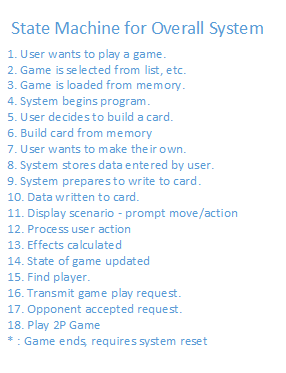
\includegraphics[width=\textwidth]{images/OSStates.png}
%		\caption{}
%		\label{fig:statesLegend}
%	\end{subfigure}
%	\caption{State diagram of the primary operating system.
%		Figure~\ref{fig:sysStates} shows the states while
%		Figure~\ref{fig:statesLegend} provides a legend}
%		\label{fig:systemStateDiagram}
%	\end{figure}
%
%	\FloatBarrier
%	\subsection{General Gameplay State Diagram\label{appendix:gameplayDiagram}}
%	\begin{figure}[H]
%		\centering
%		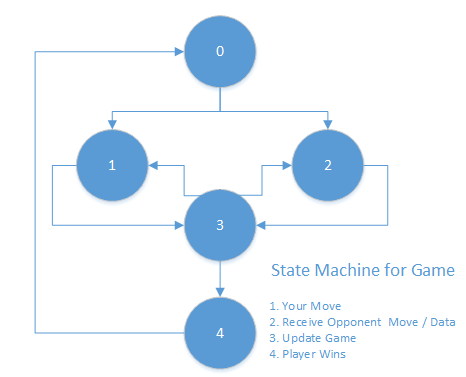
\includegraphics[width=\textwidth]{images/gamePlayState.png}
%		\caption{State diagram of basic turn-based game}
%		\label{fig:gamePlayState}
%	\end{figure}
%
%	\FloatBarrier
%	\section{Control Flow Diagrams}
%
%	\begin{figure}[H]
%		\centering
%		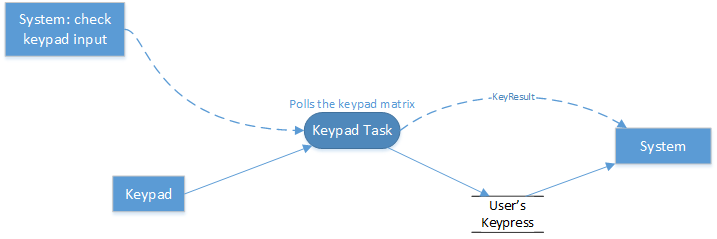
\includegraphics[width=0.75\textwidth]{images/keypadDataFlow.png}
%		\caption{Keypad response}
%		\label{fig:keypadDataFlow}
%	\end{figure}
%
%	\begin{figure}[H]
%		\centering
%		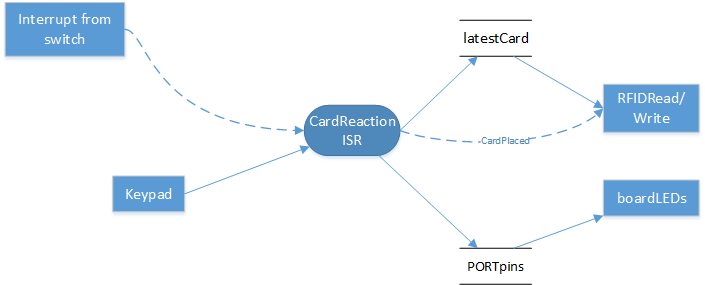
\includegraphics[width=0.8\textwidth]{images/reactionDataFlow.png}
%		\caption{Card Reaction LEDs}
%		\label{fig:cardReactionDataFlow}
%	\end{figure}
%
%	\begin{figure}[H]
%		\centering
%		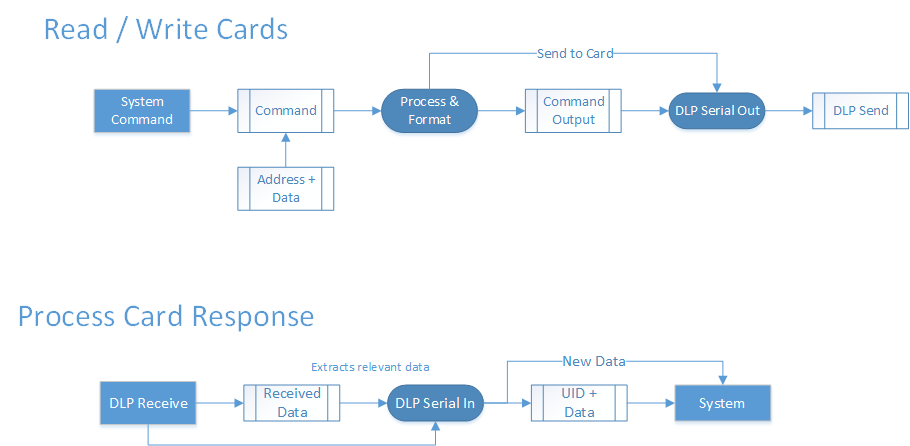
\includegraphics[width=0.8\textwidth]{images/RFIDreaderDataFlow.png}
%		\caption{RFID tag reader subsystem}
%		\label{fig:rfidDataFlow}
%	\end{figure}
%
%	\begin{figure}[H]
%		\centering
%		\begin{subfigure}{\textwidth}
%			\includegraphics[width=\textwidth]{images/I2CReceiveDataCtrlFlow.png}
%			\caption{}
%			\label{fig:i2cReceiveFlow}
%		\end{subfigure}
%
%		\begin{subfigure}{\textwidth}
%			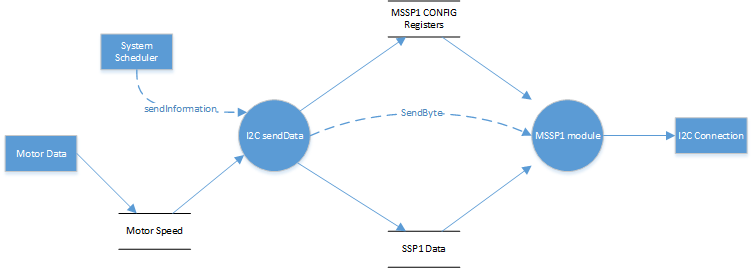
\includegraphics[width=\textwidth]{images/I2CSendCtrlFlow.png}
%			\caption{}
%			\label{fig:i2cSendFlow}
%		\end{subfigure}
%		\caption{I2C communication between microcontrollers. Figure~\ref{fig:i2cReceiveFlow} shows the flow for received data and Figure~\ref{fig:i2cSendFlow} shows the flow for transmitted data.}
%		\label{fig:i2cCtrlFlow}
%	\end{figure}
%
%	\FloatBarrier
%	\section{Project Schedule\label{appendix:ganttChart}}
%	\begin{figure}[H]
%		\centering
%		\begin{adjustbox} {rotate=90,center}
%			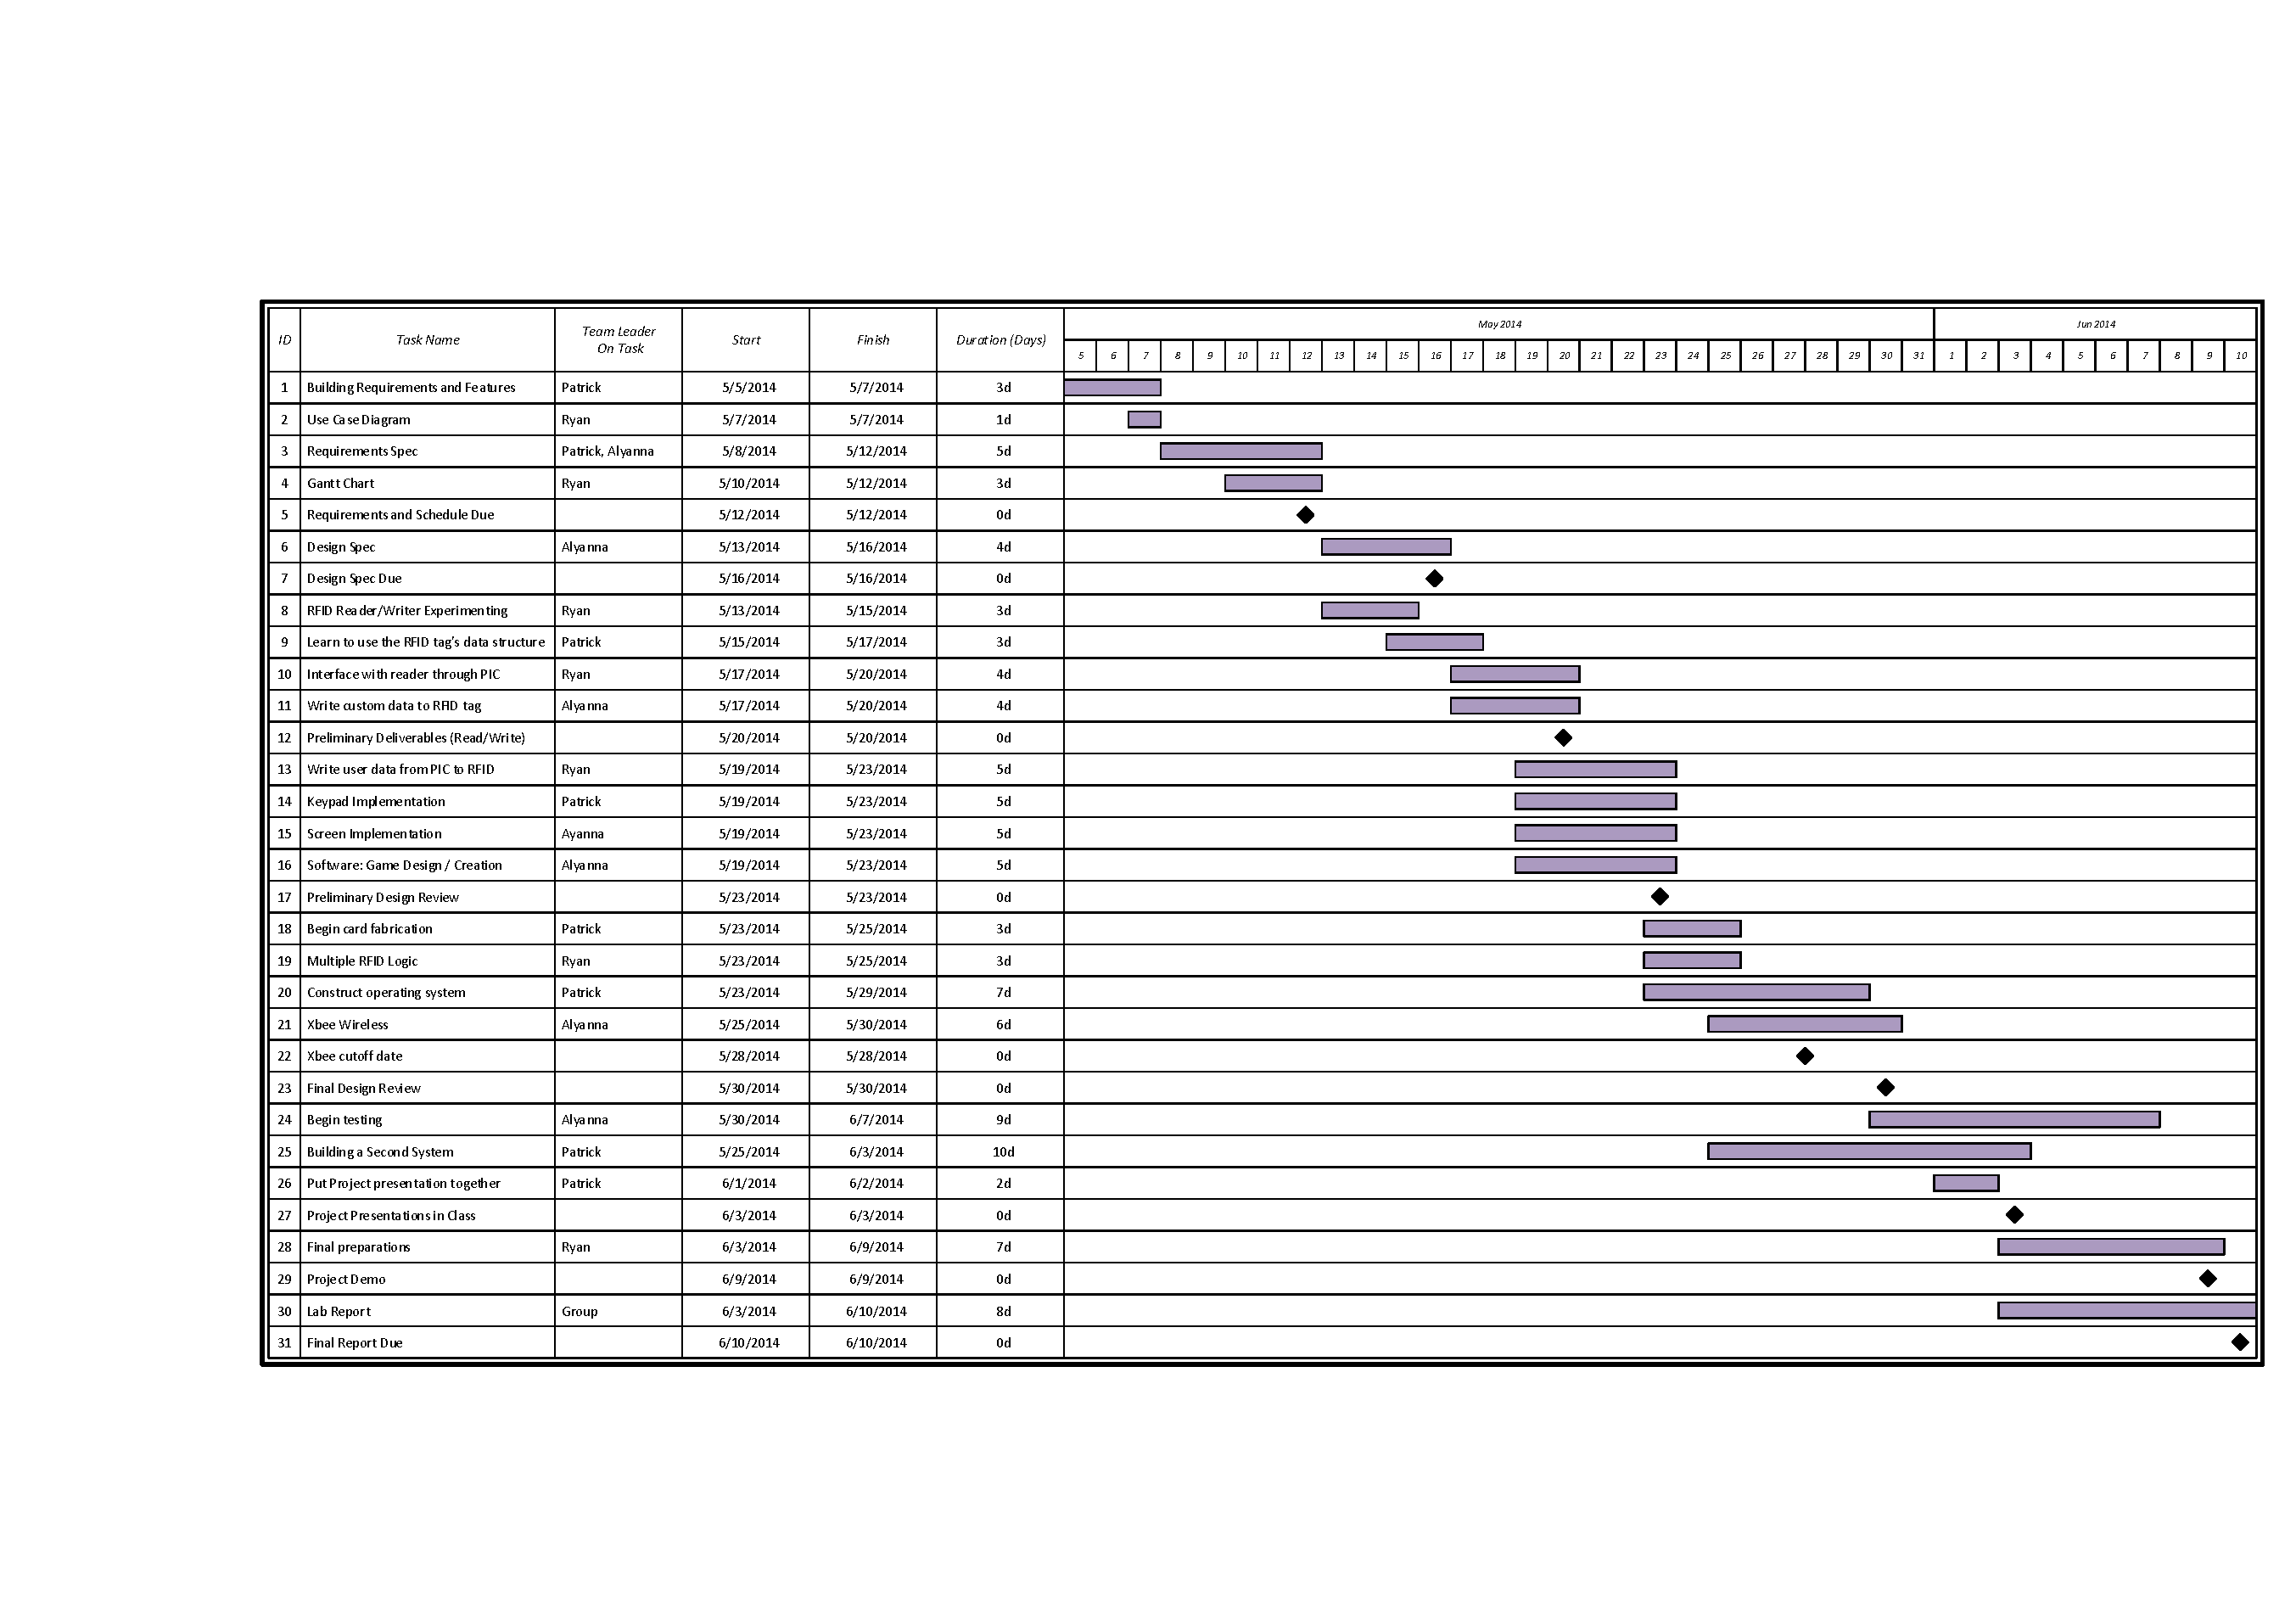
\includegraphics[width=\textwidth]{images/NewGantt.pdf}
%		\end{adjustbox}
%		\caption{Project Gantt Chart}
%		\label{fig:ganttChart}
%	\end{figure}
%
%	\clearpage
%	\section{Source Code}
%% We will put code here. Use the format:
%%    \subsection{Main Function}
%%    \lstinputlisting{../code/main.c}
%%
%%    \subsection{Tasks}
%%    \subsubsection{Task Control Blocks}
%%    \lstinputlisting{../code/tcb.h}
%	Source code for this project is provided below.
%
%	\subsection{System Scheduler}
%	The system-wide global definitions and variables are also given here for convenience.
%	\lstinputlisting{../FrontEnd.X/globals.h}
%	\lstinputlisting{../FrontEnd.X/interrupts.h}
%	\lstinputlisting{../FrontEnd.X/SchedMain.c}
%
%	\subsection{Creating Cards}
%	\lstinputlisting{../FrontEnd.X/buildCard.c}
%
%	\subsection{Example Game}
%	Both a single player and multiplayer version of the same game are provided.
%	\lstinputlisting{../FrontEnd.X/game.h}
%	\lstinputlisting{../FrontEnd.X/game.c}
%
%	\subsection{I$^2$C InterPIC Communication}
%	\lstinputlisting{../FrontEnd.X/i2cComm.h}
%	\lstinputlisting{../FrontEnd.X/i2cComm.c}
%
%	\subsection{Keypad Driver}
%	\lstinputlisting{../FrontEnd.X/keypadDriver.h}
%	\lstinputlisting{../FrontEnd.X/keypadDriver.c}
%
%	\subsection{LCD Driver}
%	\lstinputlisting{../FrontEnd.X/LCD.h}
%	\lstinputlisting{../FrontEnd.X/LCD.c}
%
%	\subsection{Card Reaction Control}
%	\lstinputlisting{../FrontEnd.X/LED.h}
%	\lstinputlisting{../FrontEnd.X/LED.c}
%
%	\subsection{Motor Driver}
%	\textit{Note: This feature was not implemented in the final product}
%	\lstinputlisting{../FrontEnd.X/motorDriver.h}
%	\lstinputlisting{../FrontEnd.X/motorDriver.c}
%
%	\subsection{RFID Reader Driver}
%	\lstinputlisting{../FrontEnd.X/rfidReader.h}
%	\lstinputlisting{../FrontEnd.X/rfidReader.c}
%
%	\subsection{EIA-232 Serial Connection}
%	\lstinputlisting{../FrontEnd.X/rs232.h}
%	\lstinputlisting{../FrontEnd.X/rs232.c}
%
%	\subsection{SRAM Primary Memory}
%	\textit{Note: There are two different files for each microcontroller due to hardware configurations}
%	\lstinputlisting{../FrontEnd.X/SRAM.h}
%	\lstinputlisting{../FrontEnd.X/SRAMfront.c}
%	\lstinputlisting{../FrontEnd.X/SRAMback.c}
%
%	\subsection{SPI Initialization}
%	\textit{Note: SPI used for communication with the LCD display}
%	\lstinputlisting{../FrontEnd.X/startup.h}
%	\lstinputlisting{../FrontEnd.X/startup.c}
%
%	\subsection{Wireless Connectivity via Xbee}
%	\lstinputlisting{../FrontEnd.X/xbee.h}
%	\lstinputlisting{../FrontEnd.X/xbee.c}
%
	\end{document}
